\documentclass[]{exam}
\usepackage{epic,array,ecltree,url,calrsfs}
\usepackage[nointegrals]{wasysym}

%These tell TeX which packages to use.
\usepackage{array,epsfig}
\usepackage{amsmath}
\usepackage{amsfonts}
\usepackage{amssymb}
\usepackage{amsxtra}
\usepackage{amsthm}
\usepackage{mlextra} % must come after ams packages
\usepackage{mathrsfs}
\usepackage[dvipsnames]{xcolor}
\usepackage{array}
\usepackage{graphicx}
\graphicspath{ {../art/} }
\usepackage{subfig}
\usepackage{bm}
\usepackage{tikz}
\usepackage{multicol}
\usepackage{enumitem}

\newcommand{\twonode}{%
  \begingroup\normalfont
  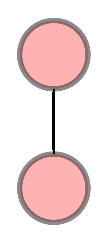
\includegraphics[height=\fontcharht\font`\b]{2nodetree.eps}%
  \endgroup
}

\newcommand{\tf}[1][{}]{%
\fillin[#1][0.25in]%
}
\title{Lab 10: Linear Temporal Logic, Applications to the Critical Section
  Problem}

\author{Foundations of Computer Science}
\date{\today}
%\pagestyle{empty} 
%\footer{}{\thepage}{}
\unframedsolutions
\SolutionEmphasis{\itshape\small}
\SolutionEmphasis{\color{NavyBlue}}


\begin{document}

\maketitle
\setlength{\columnseprule}{1pt}
\section*{Linear Temporal Logic Practice}
\begin{questions} 
\question Give counterexamples to disprove the following:
\begin{parts}
\part $\models (\Box p \implies \Box q) \implies \Box(p \implies q)$
\begin{solution}
~\\
\unitlength=.9pt
\begin{picture}(340,30)
\put(  0,-5){\state{p}{$s_{0}$}}
\put( 20, 5){\vector(1,0){40}}
\put( 60,-5){\state{}{$s_{1}$}}
\put( 80, 5){\vector(1,0){40}}
\put(120,-5){\state{}{$s_{2}$}}
\put(140, 5){\vector(1,0){40}}
\put(180,-5){\state{}{$s_{3}$}}
\put(200, 5){\vector(1,0){40}}
\put(240,-5){\state{}{$s_{4}$}}
\put(260, 5){\vector(1,0){40}}
\put(300, 0){\makebox(20,10){\ldots}}
\end{picture}

Generally: any interpretation in which $p$ is true in at least one state, but not
true in all states, and $q$ is false in the state where $p$ is true.
\end{solution}
\part $\models \Diamond(p \implies q) \implies (\Diamond p \implies \Diamond q)$
\begin{solution}
~\\
\unitlength=.9pt
\begin{picture}(340,30)
\put(  0,-5){\state{p}{$s_{0}$}}
\put( 20, 5){\vector(1,0){40}}
\put( 60,-5){\state{}{$s_{1}$}}
\put( 80, 5){\vector(1,0){40}}
\put(120,-5){\state{}{$s_{2}$}}
\put(140, 5){\vector(1,0){40}}
\put(180,-5){\state{}{$s_{3}$}}
\put(200, 5){\vector(1,0){40}}
\put(240,-5){\state{}{$s_{4}$}}
\put(260, 5){\vector(1,0){40}}
\put(300, 0){\makebox(20,10){\ldots}}
\end{picture}

Generally: any interpretation in which $p$ is true at least once and $q$ is never true.
\end{solution}
\end{parts}
\vspace{5mm}
\question Prove the following formulas are valid:
\begin{parts}
\part $\models (\Diamond p \imp \Diamond q) \imp \Diamond(p \imp q)$
\begin{solution}
\begin{proof}
The implication can only be false if the antecedent is true and the
consequent is false. To show that this is impossible, we assume $(\Diamond p \imp
\Diamond q)$ is true and show that this implies $\Diamond(p \imp q)$ cannot be 
false. Note that $\Diamond(p \imp q)$ is true as long as there is some state
in which $p \imp q$ is true. By definition of the implication, this condition is 
satisfied as long as there is some state in which both $p$ and $q$ are true, or
$p$ is false (and $q$ is either false or true).

Similarly, if $(\Diamond p \imp \Diamond q)$ is true, then either $\Diamond p$ is false,
or $\Diamond p$ is true and $\Diamond q$ is true. We consider each of these
possibilities separately: 
\begin{itemize}
\item If $\Diamond p$ is false, this implies $\Box \ngg p$---that is, $p$ is false for all states.
Consequently, $p \imp q$ is vacuously true for all states, so clearly $\Diamond (p \imp q)$.
\item If $\Diamond p$ is true and $\Diamond q$ is true, then there must be at least
one state where $p$ is true and at least one state where $q$ is true. This
creates two cases:
\begin{enumerate}
\item  If $p$ and $q$ are true in the same state, then $p \imp q$ holds for that
state, and therefore $\Diamond (p \imp q)$ is true.
\item If $p$ and $q$ are never true in the same state, then there is some state
where $p$ is false and $q$ is true. Then $p \imp q$ holds (vacuously) for that
state, and therefore $\Diamond (p \imp q)$ is true.
\end{enumerate}
\end{itemize}
\end{proof}

\end{solution}
\part $\models \Box p \imp (\Diamond q \imp \Box p)$
\begin{solution}
\begin{proof}
This formula is valid because it is a substitution instance of the valid propositional logic formula
$A \imp (B \imp A)$, where $A \equiv \Box p$ and $B \equiv \Diamond q$. 
To see this formula is valid, note $(A \imp B) \imp A$ can only be falsified if
the antecedent is true but the consequent is false. However, if the antecedent
is true then $A$ is true, so the consequent $B \imp A$ cannot be false. 
\end{proof}
\end{solution}
\part $\models \Diamond (p \land q) \lor \Box ( \ngg p \lor \ngg q)$
\begin{solution}
\begin{proof}
Observer that the right side of the formula, $\Box ( \ngg p \lor \ngg q)$,
can be rewritten as follows:
\begin{align*}
\Box ( \ngg p \lor \ngg q) &\equiv  \Box \ngg (p \land q)\\
                           &\equiv  \ngg \Diamond \ngg \ngg (p \land q)\\
                           &\equiv  \ngg \Diamond (p \land q)
\end{align*}
Substituting this back into the original formula yields:
\[
  \models \Diamond (p \land q) \lor \Box ( \ngg p \lor \ngg q)
\]
which is a substitution instance of the valid propositional logic
formula $A \lor \ngg A$, obtained by setting $A \equiv \Diamond (p \land q)$.
\end{proof}
\end{solution}
\end{parts}

\question Use Linear Temporal Logic to express the properties of liveness and
mutual exclusion.
\begin{solution}
Define $p$, $q$, $p'$ and $q'$ as follows:\\

 $p$: ``Process p is in the critical section.''\\
 $q$: ``Process q is in the critical section.''\\ 
 $p'$: ``Process p is attempting to enter the critical section.\\
 $q'$: ``Process q is attempting to enter the critical section.''\\
Then mutual exclusion can be expressed as 
\[
  \Box \ngg (p \land q)
\]
Liveness is the guarantee that if a process attempts to enter its critical section, it
will eventually succeed. This can be expressed as:
\[\Box (p' \imp \Diamond p) \land \Box (q' \imp \Diamond q)\]

\end{solution}
\uplevel{\section*{Modeling the Critical Section Problem }}
\question Consider the following alternative implementation of Peterson's algorithm:
\begin{center}
\begin{tabular}{|p{0.46\textwidth}|p{0.46\textwidth}|}
\hline
\multicolumn{2}{|c|}{\p{boolean wantp = false, wantq = false}}\\
\multicolumn{2}{|c|}{\p{int turn = 1}}\\\hline
\p{Process p} & \p{Process q} \\
\hline
\p{while (true) \{} & \p{while (true) \{} \\
\p{\ \ non-critical-section} & \p{\ \ non-critical-section} \\
\p{\ \ turn = 1} & \p{\ \ turn = 2} \\
\p{\ \ wantp = true} & \p{\ \ wantq = true} \\
\p{\ \ wait until } & \p{\ \ wait until } \\
\p{\ \ \ \ (!wantq or turn == 2)} & \p{\ \ \ \ (!wantp or turn == 1)} \\
\p{\ \ critical-section} & \p{\ \ critical-section} \\
\p{\ \ wantp = false} & \p{\ \ wantq = false} \\
\p{\}} & \p{\}} \\\hline
\end{tabular}
\end{center}

Write out a sequence of interleaved executions that demonstrates this
version of the algorithm no longer guarantees mutual exclusion.
\begin{solution}
\begin{tabular}{|l|l|l|l|}
\hline
0. & Start.                                   & State: & $wantp = false$, $wantq = false$, $turn = 1$ \\
\hline
1. & Process $p$ sets $turn$ to $1$.          & State: & $wantp = false$, $wantq = false$, $turn = 1$ \\ 
\hline
2. & Process $q$ sets $turn$ to $2$.          & State: & $wantp = false$, $wantq = false$, $turn = 2$ \\
\hline
3. & Process $q$ sets $wantq$ to $true$.      & State: & $wantp = false$, $wantq = true$, $turn = 2$ \\
\hline
4. & Process $q$ enters the critical section. & State: & $wantp = false$, $wantq = true$, $turn = 2$ \\
\hline
5. & Process $p$ sets $wantp$ to $true$.      & State: & $wantp = true$, $wantq = true$, $turn = 2$ \\ 
\hline
6. & Process $p$ enters the critical section. & State: & $wantp = true$, $wantq = true$, $turn = 2$ \\
\hline
\end{tabular}
\end{solution}

\question\label{q:delta} Consider the following transition function, $\delta$, which is fully
defined as follows:
\begin{align*}
  \delta(s_0,0) = s_0,\;\;& \delta(s_0,1) = s_1 \\
  \delta(s_1,0) = s_0,\;\;& \delta(s_1,1) = s_2 \\
  \delta(s_2,0) = s_1,\;\;& \delta(s_2,1) = s_2
\end{align*}

Evaluate $\hat{\delta}(s,w)$, for the values of $s$ and $w$ given below. For each, first rewrite $\hat{\delta}$ in terms of $\delta$:
\begin{parts}
\part $s = s_0$, $w = 10$
\begin{solution}
\begin{align*}
\hat{\delta}(s_0,10) &= \delta(\hat{\delta}(s_0,1), 0)\\ 
                     &= \delta(\delta(\hat{\delta}(s_0,\epsilon), 1),0)\\
                     &= \delta(\delta(s_0, 1),0)\\
                     &= \delta(s_1, 0)\\
                     &=  s_0
\end{align*}
\end{solution}
\part $s = s_0$, $w = 1100$
\begin{solution}
\begin{align*}
\hat{\delta}(s_0,1100) &= \delta(\hat{\delta}(s_0, 110),0)\\
                       &= \delta(\delta(\hat{\delta}(s_0, 11),0),0)\\
                       &= \delta(\delta(\delta(\hat{\delta}(s_0, 1),1),0),0)\\
                       &= \delta(\delta(\delta(\delta(\hat{\delta}(s_0,\epsilon), 1),1),0),0)\\
                       &= \delta(\delta(\delta(\delta(s_0, 1),1),0),0)\\
                       &= \delta(\delta(\delta(s_1,1),0),0)\\
                       &= \delta(\delta(s_2,0),0)\\
                       &= \delta(s_1,0)\\
                       &= s_0
\end{align*}
\end{solution}
\part $s = s_2$, $w = \epsilon$
\begin{solution}
$\hat{\delta}(s_2,\epsilon) = s_2$
\end{solution}
\end{parts}


\vspace{5mm}
\question Draw a state diagram that corresponds to the transition function in question
\ref{q:delta}, above.
\vspace{5mm}
\begin{solution}
~\\
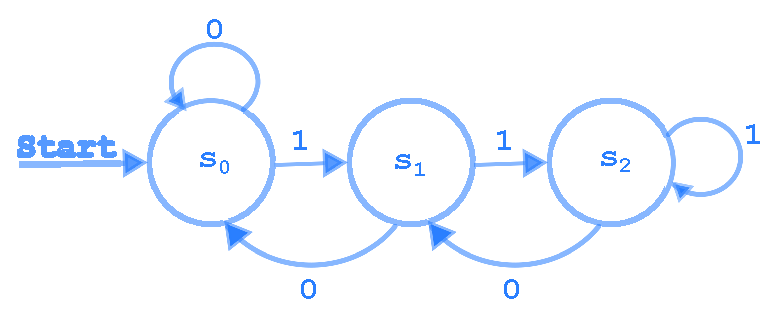
\includegraphics{lab10_automaton.eps}
%\unitlength=.9pt
%\begin{picture}(340,30)
%\put( -10,10){\vector(1,0){10}}
%\put(  0, 0){\state{$s_0$}{}}
%\put( 17,20){\oval(10,10)[r]}
%\put( 2,20){\oval(10,10)[l]}
%\put( 0,25){\line(1,0){18}}
%\put( 20,10){\vector(1,0){40}}
%\put( 60, 0){\state{$s_1$}{$s_{1}$}}
%\put( 80,10){\vector(1,0){40}}
%\put(120, 0){\state{$s_2$}{$s_{2}$}}
%\end{picture}
\end{solution}


\question\label{q:2ndattempt} Consider the following proposed solution to the critical section
problem:
\begin{center}
\begin{tabular}{|p{0.45\textwidth}|p{0.45\textwidth}|}
\hline
\multicolumn{2}{|c|}{\p{boolean wantp = false, wantq = false}}\\
\hline
\p{Process p} & \p{Process q} \\
\hline
\p{while (true) \{} & \p{while (true) \{} \\
\p{\ waitp: wait until !wantq} & \p{\ waitq: wait until !wantp} \\
\p{\ tryp: \ wantp = true} & \p{\ tryq: \ wantq = true} \\
\p{\ csp: \ wantp = false} & \p{\ csq: \ wantq = false} \\
\p{\}} & \p{\}} \\\hline
\end{tabular}
\end{center}
\begin{parts}
\part Draw the automaton for each process.
\begin{solution}
\begin{center}
\unitlength=1.1pt
\begin{picture}(230,180)
%\put(0,0){\framebox(230,180){}}
%process p
\put(0,160){
\put(0,0){
  \put(-20,15){\vector(1,0){18}}
  \put(15,15){\circle{30}}
  \put( 0, 0){\makebox(30,30){\p{waitp}}}
  \put(32,15){\vector(1,0){66}}

  \put(28,32){\oval(26,20)[r]}
  \put(2,32){\oval(26,20)[l]}
  \put(28,42){\line(-1,0){26}}
  \put(-3,22){\vector(1,0){5}}
  \put(-25,42){
     \makebox(70,20){\p{wantq==true}}
  }
  \put(28,0){
     \makebox(70,20){\p{wantq==false}}
  }
}
\put(100,0){
  \put(15,15){\circle{30}}
  \put( 0, 0){\makebox(30,30){\p{tryp}}}
  \put(32,15){\vector(1,0){66}}
  \put(28,0){
     \makebox(70,20){\p{wantp = true}}
  }
}
\put(200,0){
  \put(15,15){\circle{30}}
  \put( 0, 0){\makebox(30,30){\p{csp}}}
  \put(15,-2){\line(0,-1){38}}
  \put(15,-40){\line(-1,0){200}}
  \put(-185,-40){\vector(0,1){38}}
  \put(-120,-43){
     \makebox(70,20){\p{wantp=false}}
  }
}
}

% process q
\put(0,40){
\put(0,0){
  \put(-20,15){\vector(1,0){18}}
  \put(15,15){\circle{30}}
  \put( 0, 0){\makebox(30,30){\p{waitq}}}
  \put(32,15){\vector(1,0){66}}

  \put(28,32){\oval(26,20)[r]}
  \put(2,32){\oval(26,20)[l]}
  \put(28,42){\line(-1,0){26}}
  \put(-3,22){\vector(1,0){5}}
  \put(-25,42){
     \makebox(70,20){\p{wantp==true}}
  }
  \put(28,0){
     \makebox(70,20){\p{wantp==false}}
  }
}
\put(100,0){
  \put(15,15){\circle{30}}
  \put( 0, 0){\makebox(30,30){\p{tryq}}}
  \put(32,15){\vector(1,0){66}}
  \put(28,0){
     \makebox(70,20){\p{wantq = true}}
  }
}
\put(200,0){
  \put(15,15){\circle{30}}
  \put( 0, 0){\makebox(30,30){\p{csq}}}
  \put(15,-2){\line(0,-1){38}}
  \put(15,-40){\line(-1,0){200}}
  \put(-185,-40){\vector(0,1){38}}
  \put(-120,-43){
     \makebox(70,20){\p{wantq=false}}
  }
}
}
\end{picture}
\end{center}
\end{solution}


\part\label{q:mutexfail} Write out a sequence of interleaved executions which results
in both processes being in the critical section at the same time. 
\begin{solution}
\begin{tabular}{|l|l|l|l|}
\hline
0. & Start.                                   & State: & $wantp = false$, $wantq = false$ \\
\hline
1. & Process $p$ enters $tryp$.               & State: & $wantp = false$, $wantq = false$ \\ 
\hline
2. & Process $q$ enters $tryq$.               & State: & $wantp = false$, $wantq = false$ \\
\hline
3. & Process $p$ sets $wantp$ to $true$ and enters $csp$.      & State: & $wantp = true$, $wantq = false$  \\
\hline
4. & Process $q$ sets $wantq$ to $true$ and enters $csp$.     & State: & $wantp = true$, $wantq = true$  \\
\hline
\end{tabular}
\end{solution}


\part Let $\delta_p$ and $\delta_q$ be the transition functions for process
$p$ and process $q$.
\begin{subparts}
\subpart Let $\delta_p(tryp, a) = l_p$, where $a$ represents the state $wantp\land
\ngg wantq$. Find $l_p$.
\begin{solution}
$l_p = csp$
\end{solution}

\subpart Let $\delta_q(tryq, a) = l_q$, where $a$ represents the state $wantp\land
\ngg wantq$. Find $l_q$.
\begin{solution}
$l_q = tryq$
\end{solution}

\subpart Assume $\delta_p(waitp,a) = tryp$. List all possible values of $a$.
\begin{solution}
$a = wantp\land \ngg wantq$ or $a = \ngg wantp\land \ngg wantq$

\end{solution}

\subpart Complete the following definition for $\delta_p$ (You may omit combinations 
    of locations and states that do not correspond to any transition.):
\begin{gather*}
\begin{align*}
  &\delta_p(waitp,wantp\land \ngg wantq) &= \fillin\\
  &\delta_p(waitp, \fillin) &= \fillin \\
  &\delta_p(\fillin, \fillin) &= \fillin \\
  &\delta_p(\fillin, \fillin) &= \fillin 
\end{align*}\\
   \vdots\\
   etc.
\end{gather*}
\begin{solution}
\begin{align*}
  &\delta_p(waitp, wantp\land \ngg wantq)      = tryp\\
  &\delta_p(waitp, \ngg wantp\land \ngg wantq) = tryp \\
  &\delta_p(waitp, wantp\land wantq)           = waitp \\
  &\delta_p(waitp, \ngg wantp\land wantq)      = waitp \\
  &\delta_p(tryp,  wantp\land wantq)           = csp \\
  &\delta_p(tryp,  wantp\land \ngg wantq)      = csp \\
  &\delta_p(csp,   \ngg wantp\land wantq)      = waitp \\
  &\delta_p(csp,   \ngg wantp\land \ngg wantq) = waitp 
\end{align*}\\



\end{solution}

\end{subparts}
\part Find $w$ such that $\hat{\delta_p}(waitp, w) = csp$ and
$\hat{\delta_q}(waitq, w) = csq$.
\end{parts}
\begin{solution}
Using commas to separate states, one possible value of $w$ is:
\[w = \ngg wantp\land \ngg wantq,\ngg wantp\land \ngg wantq,\ngg wantp\land \ngg
wantq,wantp\land \ngg wantq,wantp\land wantq\]
(This follows the state sequence in the solution given to problem
\ref{q:2ndattempt}\ref{q:mutexfail}, above.)
\end{solution}

\end{questions}
\end{document}


